\appendix
% \appendixpage
% \addappheadtotoc

% This is tha appendix, where we may insert detailed mathematical proccedures or other data which may be useful but also will make the main
% text too large so this should be consulted only in case of neccesity

\section{Estimation of distances to meteors}
\label{app:distance}
The distance between the GOES satellite and the meteor, neccesary to estimate the radiated energy is calculated as follows:

\begin{align}
  R = \left|\vec{r}_{GLM} - \vec{r}_{obj} \right|
\end{align}

where $\vec{r}_{GLM}$ is the vector position of the GLM satellite and $\vec{r}_{obj}$ is the vector position of the meteor.

In cartesian coordinates, the distance $R$ is given by:

\begin{align}
  R &= \left((x_{GLM}-x_{obj})^2 + (y_{GLM}-y_{obj})^2 + (z_{GLM}-z_{obj})^2\right)^{1/2} \label{eq:R}\\
\end{align}

The transformation to spherical coordinates is given by:

\begin{align}
  x = r\cos\phi\cos\theta \label{eq:xtoR}\\
  y = r\sin\phi\cos\theta \label{eq:ytoR}\\
  z = r\sin\theta \label{eq:ztoR}
\end{align}

Where $r$ is measured from the center of the earth, $ -180^\circ < \phi <= 180^\circ$ represents the longitude; is positive at east of Greenwich meridian, and negative eastwards. $\-90^\circ <= \theta <= 90^\circ$ represents the latitude and is positive at the north of equator and negative southwards.

Substituting the transform (\ref{eq:xtoR} - \ref{eq:ztoR}) into (\ref{eq:R}), using elemental trigonometry and considering both GLM satellites lie into the equator ($\theta_{GLM}=0$) we get:

\begin{align}
  R^2 &= r_{GLM}^2 + r_{obj}^2 - 2r_{GLM}r_{obj}f(\theta_{obj}, \phi_{obj}, \phi_{GLM}) \label{eq:R2}\\
  \mathrm{where:} & f(\theta_{obj}, \phi_{obj}, \phi_{GLM}) = \cos\theta_{obj}\cos\left(\phi_{GLM}-\phi_{obj}\right)
\end{align}

Since $r_{GLM}$ and $r_{obj}$ are measured from the center of the earth we find that:

\begin{align}
  r_{GLM} &= r_{earth} + h_{GLM} \label{eq:rg}\\
  r_{obj} &= r_{earth} + h_{obj} \label{eq:ro}
\end{align}

Substituting (\ref{eq:rg}, \ref{eq:ro}) into \ref{eq:R2} and considering that $h_{obj} \ll h_{GLM}$ we get:

\begin{align}
  \begin{split}
    R^2 = 2r_{earth}^2\left(1-f(\theta_{obj}, \phi_{obj}, \phi_{GLM})\right) +2r_{earth}h_{GLM}\\
    \left(1-f(\theta_{obj}, \phi_{obj}, \phi_{GLM})\right) + h_{GLM}^2 - 2h_{GLM}h_{obj}f(\theta_{obj}, \phi_{obj}, \phi_{GLM})
    \end{split}
\end{align}

\section{Energy estimation}
\label{app:energy}
The total radiant energy emmited is calculated integrating over all the time and all directions. The first is obtained simply summing all the light curve points. In the other hand, to integrate over all directions, we multiply the GLM event energies by the factor (\SI{1.695e18}{})(\SI{1.018e3}{})$\left(\frac{R}{35780~km}\right)^2$ \citep{Jenniskens:2018}. This factor also considers that the GLM only detects light from the OI line. Then, we obtain the luminous efficiency $\tau_1$ (i.e the fraction of the total energy converted into radiation) following \citet{Brown:2002}:
\begin{align}
  \tau_1 = (0.1212\pm 0.0043)E_0^{0.115\pm 0.075}
\end{align}

Where $E_0$ is the luminous energy calculated from integrating GLM reported energies (in kilotons). Finally the total estimated energy is $E = E_0/\tau_1$. We may compare the resulting GLM energies with the energies reported by USG sensors using the events which belong to both samples, and we noticed that the energies obtained with GLM data is systematically lower than the energies reported by the USG sensors. In this work we assumed that this discrepancy is due to the GLM sensors does not detect the full meteor paths, just a fraction of the total radiated energy. To solve this problem we made a linear fit between the derived energies and the energies reported in the USG sample for the events which appear in both samples, and recallibrate the energies of the rest of the GLM sample. The linear fit is shown in figure \ref{fig:lin_fit}. We used the linear fit slope as the recallibration factor and the residuals as the error, we neglected the y-intercept term because this term is much larger than the most energies in the GLM sample and strongly affects the recallibrated energy.

\begin{figure}
  \centering
  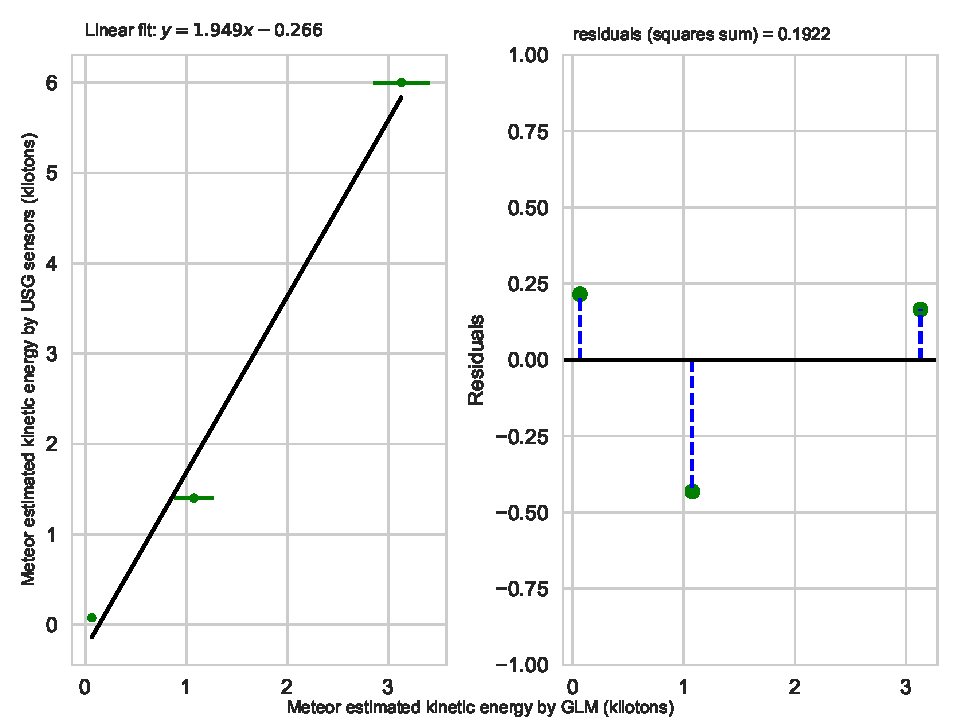
\includegraphics[width=\linewidth]{../figures/energy_fit}
  \caption{Left: Linear fit between energies calculated from GLM data and energies reported by USG sensors. Right: Residuals of the fit, used as error in the recallibration factor. The three events used for this linear fit are GLM-00 (the cuban meteoroid), GLM-23 and GLM-Ven (Venezolan meteoroid).}
  \label{fig:lin_fit}
\end{figure}


